\section{Einführung in die Energiewirtschaft}

\textbf{Energiewirtschaft}: Einrichtungen und Handlungen mit dem Ziel, die Versorgung von Haushalten und Betrieben mit Energieträgern sicherzustellen

\textbf{Umrechnung von Einheiten:} \textit{siehe Tut 1}
\begin{center}
	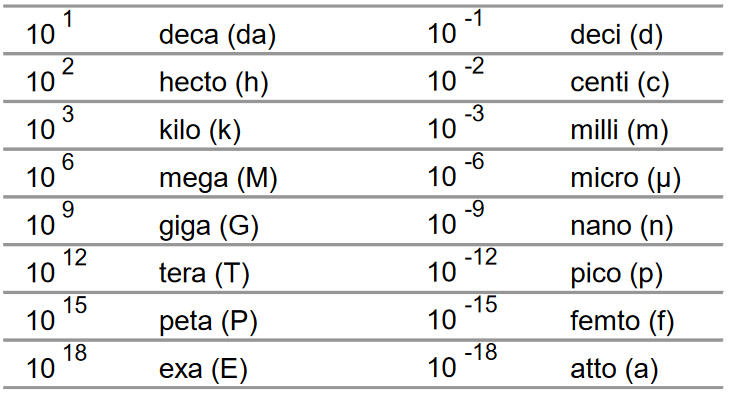
\includegraphics[width=0.5\textwidth]{images/units.png}
\end{center}

\textbf{Definitionen:}
\begin{itemize}
	\item \textbf{Energieträger}: Stoffe, aus denen oder nach deren Umwandlung Energie gewonnen werden kann
	\item \textbf{Primärenergie}: Nutzbarer Energiegehalt von Primärenergieträgern, die in der Natur vorkommen und noch keiner Umwandlung unterworfen sind
	\item \textbf{Sekundärenergie}: Energie, die als Ergebnis eines Umwandlungsprozesses und unter Energieverlust aus der Primärenergie gewonnen wird
	\textbf{Endenergie}: Dem Endverbraucher zur Verfügung stehende Energie
	\item \textbf{Nutzenergie}: Energie, die nach der letzten Umsetzung in den Geräten des Verbrauchers zur Verfügung steht
	\item \textbf{Energiedienstleistung}: Leistungen, die durch Einsatz der Nutzenergie beim Kunden erfüllt werden, z.B. Personentransport oder Raumausleuchtung
\end{itemize}
\begin{center}
	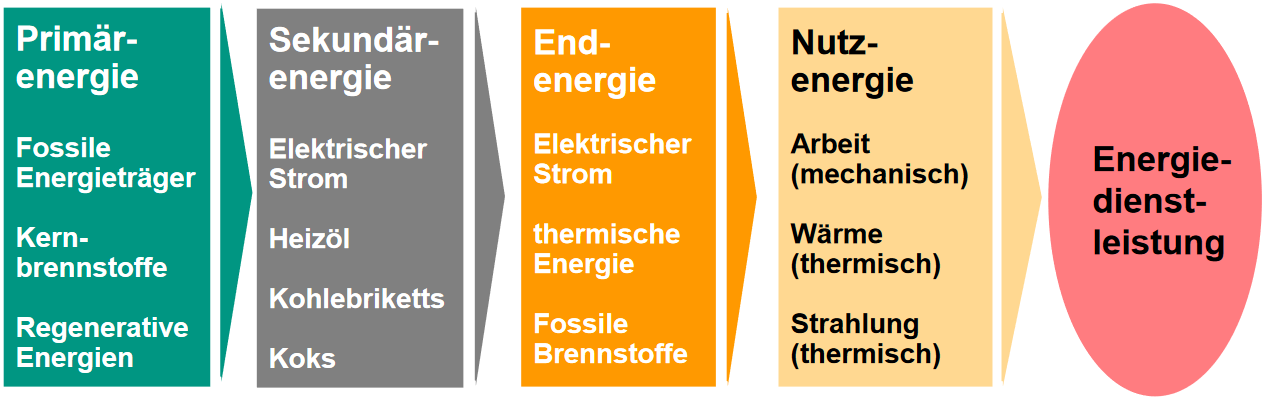
\includegraphics[width=0.6\textwidth]{images/energy-chain.png}
\end{center}